\documentclass[eng,printmode]{mgr}
\usepackage{polski}
\usepackage{url}
\usepackage[utf8]{inputenc}
\usepackage[T1]{fontenc}
\usepackage{scrextend}
\usepackage{graphicx}
\usepackage{subfigure}
\usepackage{psfrag}
\usepackage{float}
\usepackage{amsmath}
\usepackage{amsfonts}
\usepackage{enumitem}
\usepackage{supertabular}
\usepackage{array}
\usepackage{tabularx}
\usepackage{hhline}
\usepackage{graphicx}
\graphicspath{ {./img/} }
\usepackage{showlabels}
\usepackage{lmodern}
\usepackage{tabu}

\usepackage{listings}
\usepackage{color}

\definecolor{dkgreen}{rgb}{0,0.6,0}
\definecolor{gray}{rgb}{0.5,0.5,0.5}
\definecolor{mauve}{rgb}{0.58,0,0.82}

\lstset{frame=tb,
  language=python,
  aboveskip=3mm,
  belowskip=3mm,
  showstringspaces=false,
  columns=flexible,
  basicstyle={\scriptsize\ttfamily},
  numbers=none,
  numberstyle=\tiny\color{gray},
  keywordstyle=\color{blue},
  commentstyle=\color{dkgreen},
  stringstyle=\color{mauve},
  breaklines=true,
  breakatwhitespace=true,
  tabsize=3
}


\newcommand{\R}{I\!\!R}
\newtheorem{theorem}{Twierdzenie}[section]

\title{Porównanie metod wykrywania obserwacji odstających w danych teleinformatycznych}
\engtitle{Comparsion of outliers detecting methods in ICT data}
\author{Maciej Bakowicz}
\supervisor{prof. dr hab. inż. Krzysztof Walkowiak, W-4}

\field{Teleinformatyka (TIN)}
\specialisation{Projektowanie Sieci Teleinformatycznych (TIP)}


\begin{document}
\bibliographystyle{plain}
\maketitle 

\tableofcontents 

\chapter{Wstęp}  
Obserwację odstającą można zdefiniować jako punkt lub zbiór punktów, które swoimi wartościami różnią się od wartości punktów je otaczających. Obserwację taką można definiować lokalnie, gdzie anomalie to pojedyncze punkty a zbiorem porównawczym są punkty w bliskim sąsiedztwie lub bardziej globalnie, gdzie do analizy konkretnych przedziałów potrzebna jest wiedza o całym zbiorze (np. analiza miesięcznego trendu w danych ze stemplem czasowym). 
\\ \\
Występowanie danych odstających (anomalii, outliers) jest jednym z najczęściej spotykanym problemem w środowisku zajmującym się zbieraniem oraz analizą danych. Każde przeprowadzone badanie posiada odchyły w danych, miejsca, które nie pasują do ogólnie ukształtowanego trendu. Widać to szczególnie w środowiskach mniej kontrolowanych, takich, w których występowanie czynników zewnętrznych jest duże i nieprzewidywalne (duży rozrzut losowości). \\ \\
Występowanie tego typu anomalii ma negatywny wpływ na proces analizy i przygotowania takiego zbioru danych. Powoduje to bowiem, że rozkład zbioru danych jest przekłamany - z powodu występowania zawyżeń lub zaniżeń takich miar jak średnia czy mediana. Z punkty widzenia statystyki nieciągły, niejednorodny czy też niespójny zbiór danych nie może być wiarygodny i rzetelny \cite{outliers-impact}.
\\ \\
Kolejnym powiązanym problem jest problem zarządzania wykrytymi już anomaliami. Zazwyczaj stosuje się dwie metody: próba naprawienia punktu lub jego usunięcie. W zależności od charakteru i genezy danych można wykonać obie operacje, jedną z nich lub żadną. Podjęcie takiej decyzji wiąże się bezpośrednio z tym co jest badane oraz do czego tego typu zbiór danych będzie wykorzystywany. \\
Naprawa zazwyczaj polega na wykorzystaniu statycznych miar takich jak wartość średnia, mediana czy odchylenie standardowe. Istnieje wiele sprawdzonych i opublikowanych metod do tego służących. \\
Zazwyczaj do naprawy i usunięcia potrzebna jest konkretna wiedza o prawdopodobnych i dozwolonych wartościach w zbiorze. Innymi słowy, sama algorytmiczna klasyfikacja punktu jako odstającego nie jest wystarczająca, żeby podjąć jakiekolwiek kroki mające na celu ingerencję w zbiór danych. 
\\ \\ 
Ze względu na specyfikę danych w pracy nie zostanie podjęta jakakolwiek próba ingerencji w zbiór danych w celu naprawy / usunięcia.

\section{Cel pracy}
Celem niniejszej pracy jest zaprojektowanie oraz zaimplementowanie systemu, który w efektywny sposób wykryje błędy (tu: znaczące odstępstwa od normy w przedziale lokalnym) w danych tyczących się infrastruktury teleinformatycznej (głównie stacje nadawczo-odbiorcze BTS - Base Transceiver Station). W czasie realizacji pracy zostaną zaimplementowane istniejące oraz własne algorytmy a następnie porównane między sobą w celu wybrania sposobu (algorytmu) optymalnego. Zaprojektowany system nie powinien sam ingerować w dane (usuwać, zmieniać), gdyż dane nie są obarczone informacjami dodatkowymi (jak chociażby przerwy w działaniu stacji bazowych) przez co nie ma wystarczającej wiedzy potrzebnej do stwierdzenia przyczyny wystąpienia błędu. W końcowej fazie projektu system powinien móc wskazać błędne dane a następnie przedstawić użytkownikowi możliwości, gdzie w zależności od natury, charakteru użytkownik mógłby je usunąć lub spróbować naprawić (ręcznie lub za pomocą algorytmów uczenia maszynowego). 

\section{Zakres pracy}
\subsection{Przygotowanie danych}
Pierwszym etapem niniejszej pracy jest zebranie rzeczywistych danych od firmy zajmującej się ich zbieraniem i przetwarzaniem.  \\
Wartości oraz opisy pewnych cech tych danych są w dużej mierze tajne i zawierają poufne informacje, dlatego przedstawienie ich w niezmienionej formie byłoby poważnym naruszeniem umowy oraz klauzuli poufności zawartych z firmą. \\
Dlatego kolejnym krokiem jest zaprogramowanie algorytmu, programu, który będzie w stanie zmienić strukturę tych danych, w szczególności przypisać nazwy rzeczywistych operatorów oraz identyfikatorów urządzeń zbierających dane do nazw losowych, którymi posługiwać będzie można się w sposób swobodny w dalszych etapach pracy. \\
Zdobyte dane zawierają również szereg dodatkowych informacji, które powinny zostać odrzucone ze względu na małą wartość informacyjną i zachowanie ich jest niepotrzebne do realizacji celu pracy. Dlatego kolejnym i ostatnim krokiem w przygotowaniu danych jest stworzenie nowych struktur, tabel i schematów a następnie przekopiowanie tych wartości, które są niezbędne. Ilość danych (około pół miliona wierszy) jest na tyle duża, że wykorzystanie mechanizmów do zarządzania Big Data jest niezbędne \cite{cassandra}\cite {cassandra-driver}.

\subsection{Wybór technologii i algorytmów}
Po utworzeniu struktur i wypełnieniu ich danymi kolejnym krokiem jest wybranie istniejących już algorytmów wykrywania obserwacji odstających \cite{outliers-basic} a następnie ich implementacja w wybranym języku programistycznym lub wykorzystanie rozwiązań już wcześniej zaimplementowanych. Ilość zaimplementowanych algorytmów zależy w dużej mierze od stopnia trudności w ich implementacji oraz testowaniu a także od ilości dostępnych materiałów na ich temat. W obrębie wyboru algorytmów znajdzie się zatem nie tylko ich wyszukanie i implementacja ale także wstępna segregacja wraz z odrzuceniem tych mniej obiecujących czy nie pasujących do koncepcji. Część zaimplementowanych algorytmów może w końcowym etapie nie być brane pod uwagę ze względu właśnie na ich mniejszą użyteczność. \\
Najbardziej obiecującą technologią jest język Python \cite{python} ze względu na dużą ilość bibliotek do tworzenia struktur i schematów danych \cite{pandas} a także działań matematycznych co uproszcza proces pisania algorytmów \cite{numpy}.

\subsection{Napisanie własnego algorytmu}
Po zaimplementowaniu i przetestowaniu istniejących już rozwiązań oraz analizie ich wyników zostanie zaimplementowany własny algorytm, który wykorzystuje autorskie rozwiązania. Aby w procesie porównywania algorytmów wyniki były rzetelne i porównywalne rozwiązania te muszą wykorzystywać podobne mechaniki co wcześniej wybrane algorytmy \cite{isolation-forest}\cite{novelty}. 

\subsection{Stworzenie raportu porównawczego}
Końcowym etapem pracy jest napisanie raportu porównawczego oraz wybór cech, które będą ze sobą porównywane. Raport ten zawiera szereg porównań między kolejnymi algorytmami wraz ze wskazaniem tego optymalnego w zależności od przypadku użycia. Algorytmy są testowane kilkukrotnie na różnych zestawach danych (różniącymi się charakterystykami oraz wartościami). \\
Na potrzeby lepszej wizualizacji porównań oraz działania poszczególnych algorytmów do raportu zostaną dołączone spore ilość wykresów, data gramów oraz tabel.

\chapter{Przegląd literatury}
Specyfika dostarczonych danych, które są wykorzystywane do przeprowadzenia badań i symulacji wybranych metod narzuca pewne ograniczenia co do wyboru i wykorzystania algorytmów. Z powodu braku jakichkolwiek wzorcowych zbiorów danych, które mogłyby posłużyć jako zbiory uczące. \\
Wybrane algorytmy zatem powinny mieć możliwość klasyfikacji zbioru danych (podziału wg. określonych cech) a następnie na podstawie określonego warunku i parametrów określały punkty odstające.

\section{Metoda okna czasowego}
Metoda okna czasowego jest to sposób podziału całego zbioru danych na szereg mniejszych zbiorów zawierających się w pojedynczym, z góry określonym wycinku czasowym (dziedzina funkcji).\\
Podział określają dwa parametry:
\begin{itemize}
\item \textbf{szerokość okna} - ilość punktów dla podzbiorów wygenerowanych z podanego zbioru danych
\item \textbf{długość kroku} - ilość punktów o które okno jest przesuwane w każdej iteracji
\end{itemize}

Startowa pozycja okna to punkt 0 na osi X (dziedzina). Okno przesuwa się w prawą stronę. Dopuszczalne jest aby ostatni podzbiór miał inną szerokość niż przyjęta na początku (wynika to z niekoniecznie całkowicie podzielnego zbioru danych na równe podzbiory).
\\ \\
Działanie metody wizualizuje poniższy rysunek:

\begin{figure}[H]
  \begin{center}
  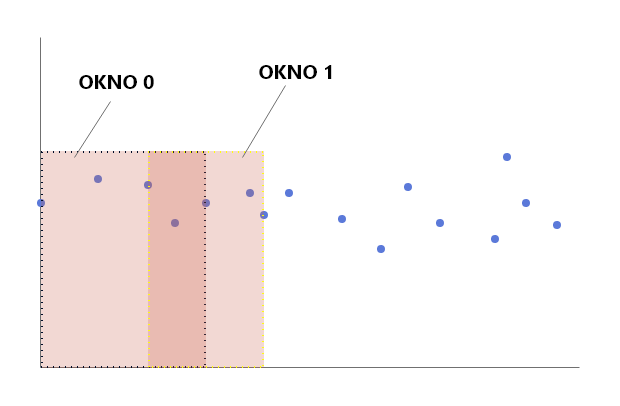
\includegraphics[scale=0.7]{okno_czasowe}
  \end{center}
  \caption{Działanie metody podziału na okna czasowe}
\end{figure}


Szerokość okna przyjęto jako 5 a długość kroku jako 2. Można zauważyć, że okna różnią się obszarem zajmowanej dziedziny co wynika z niejednorodnego rozrzutu punktów.
\\
Dodatkowo widać, że istnieją części wspólne dla sąsiadujących podzbiorów. Zastosowanie okna czasowego w tej postaci, zapewni, że większość punktów może być analizowana w różnych środowiskach, przez co eliminuje się lokalne odchylenia, istniejące jedynie w jednym z podzbiorów.
\\
W zależności od zastosowanego algorytmu na podzbiorach metoda ta powinna dzielić zbiór danych na co najmniej 10 podzbiorów lecz należy pamiętać, że ilość punktów w danym podzbiorze (szerokość okna) nie powinna być mniejsza niż 2-5 procent szerokości całego zbioru danych.
\\
Zastosowanie tej metody zatem jest opłacalne jedynie, gdy badany zbiór danych posiada sporą ilość wartości (liczonych w setkach). Dla mniejszych zbiorów danych stosowanie tej metody nie ma sensu. 

\section{Algorytm K-Mean}
Algorytm opierający swoje działanie na podziale zbioru danych na podzbiory nazywane klastrami (ang. clusters). Przydział punktów do konkretnego klastra polega na obliczaniu jego odległości względem punktów sąsiednich (odległość euklidesowa). \\ \\
Algorytm przyjmuje wiele parametrów, jednak najważniejszym jest ilość klastrów, na które należy podzielić zbiór danych.

Podział na klastry definiuje również pojęcie centroidów (ang. centroids), które przyjmują wartości środka wyznaczonych klastrów (każdy klaster posiada jeden centroid). \\ \\

Podział serii danych ze stemplem czasowym na pojedyncze klastry wraz z centroidami można zobaczyć na poniższym rysunku:

\begin{figure}[H]
  \begin{center}
  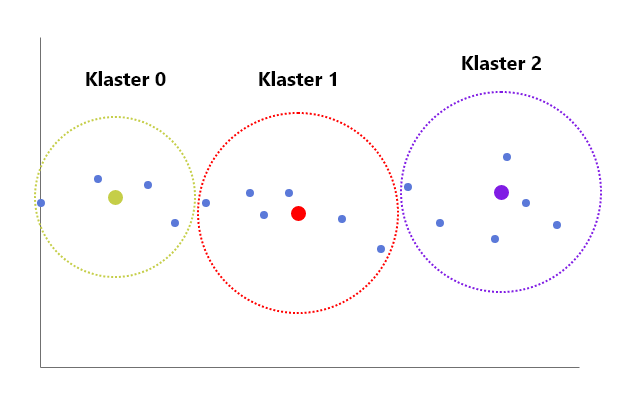
\includegraphics[scale=0.7]{KMean}
  \end{center}
  \caption{Klasyfikacja zbioru danych}
\end{figure}

Informację o przynależności punktu do konkretnego klastra można wykorzystać do wyznaczenia punktów odstających lokalnie (w jednym klastrze). \\
Sam stempel czasowy jest cechą słabą (jest ona różna dla każdego punktu), dlatego przy stosowaniu tej metody należy rozważyć przypisanie cech dodatkowych, dzięki którymi podział na klastry będzie bardziej dokładniejszy.
\subsection{Wykorzystanie odległości od centroidu}
Jednym ze sposobów określania punktu jako odstającego jest obliczenie odległości w układzie współrzędnych tego punktu od centroidu klastra, do którego ten punkt należy. Następnie można wyznaczyć punkty odstające na dwa sposoby:
\begin{itemize}
\item \textbf{odrzucić punkty powyżej zadanego progu} - z zadanym warunkiem odrzucenia, wszystkie punkty, które przekraczają próg warunku zostają sklasyfikowane jako odstające. Metoda wymaga dodatkowych obliczeń takich jak wartość środkowa wartości w każdym klastrze w celu określenia punktu odniesienia. Warunek może przyjąć różne formy, lecz zazwyczaj opiera się on na proporcji względem wartości w zbiorze (np. przekroczenie dwukrotnej wartości średniej lub stosunek wartości średniej do wartości liczonego punktu).
\item \textbf{odrzucić punkty najbardziej odległe} - trochę prostsza metoda, zakłada, że każdy zbiór danych zawiera pewne ilości punktów odstających, dlatego klasyfikuje najbardziej oddalone punkty jako odstające (biorąc pod uwagę wszystkie punkty, ze wszystkich klastrów, posortowane wartościami odległości od swoich centroidów). Ilość wybranych punktów jest zadana z góry, zazwyczaj około 5-10. Można by zakładać, że takie podejście jest niepoprawne, dlatego rekomenduje się przeprowadzenie wielokrotnych przeliczeń tego samego zbioru danych a następnie uśrednienie wartości otrzymanych (np. przeprowadzenie kilkukrotnych iteracji a następnie uwzględnienie punktów jako dostające jedynie wtedy, gdy wystąpiły one w 90 procentach przeprowadzonych iteracji)  \cite{kmean_dist}. 
\end{itemize}
\subsection{Wykorzystanie całych klastrów}
Kolejną metodą wykorzystującą algorytm klasteryzacji KMean jest metoda klasyfikująca całe klastry jako odstające. Wynika to z założenia, że testowe zbiory danych mogą zawierać pewne przedziały mocno niepasujących, pojedynczych danych (klaster bardzo odległy od pozostałych klastrów). Jeśli zatem klaster zawiera znacznie małą ilość punktów (w porównaniu do ilości zdefiniowanych klastrów oraz wielkości zbioru danych) to istnieje duże prawdopodobieństwo, że zawiera on jedynie punkty odstające. \\\\
Metoda defniuje dodatkowy parametr opisujący procentową liczbę punktów zawartych w klastrze jako warunek, na podstawie którego stwierdzana jest klasyfikacja klastra jako całego zbioru punktów odstających.
\\\\
Tak sklasyfikowany zbiór przedstawia poniższy rysunek:
\begin{figure}[H]
  \begin{center}
  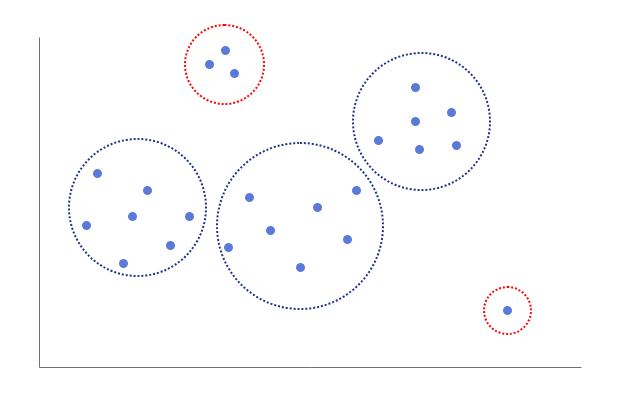
\includegraphics[scale=0.7]{KMean_sim}
  \end{center}
  \caption{Podział na klastry z różną ilością punktów wewnątrz}
\end{figure}
Jak można zauważyć klastry zaznaczone na czerwono zawierają małą ilość punktów (mniejszą niż pozostałe klastry). Metoda oznaczy wszystkie punkty w tych klastrach jako odstające.
\\\\
Geneza metody wynika z pewnej wiedzy o prawdopodobnych wystąpieniach punktów odstających w otrzymanych zbiorach danych i jest w pełni autorska (nie uwzględniając algorytmu KMean).

\section{Algorytm regresji liniowej}
Algorytm regresji liniowej jest najprostszym z wybranych algorytmów. Na zadanym zbiorze danych wyznaczana jest prosta regresji za pomocą metody najmniejszych kwadratów, czyli funkcja liniowa reprezentująca oszacowane wartości bazując na zadanym zbiorze danych. 
\\\\
Dla każdego punktu czasowego linia regresji wyznacza pewną wyestymowaną wartość. Różnica wartości tego punktu oraz punktu aktualnego (ze zbioru danych) jest nazywana błędem.
\\\\
Znając wartość błędu oraz zadając warunek można wyznaczyć punkty odstające. Wystarczy jedynie odrzucić te, których błąd jest największy (lub przekracza zadany próg, podobnie jak w metodzie KMean wykorzystującą wartość odległości od centroidu).
\\\\
Metoda ta ma jednak pewną wadę. Idealnymi zbiorami danych, dla których można tę metodę wykorzystać są te, które mają pewien zadany na początku, niezmieniający się trend. W momencie gdy występują różnice lokalne między maksymalnymi i minimalnymi wartościami lub obserwuje się miejsca "wyciszenia" (zakresy czasowe, gdzie wartości są zerowe lub bliskie zeru) metoda ta będzie generować zbyt dużą ilość błędów, żeby w efektywny sposób wyznaczyć pojedyncze punkty (zamiast tego będą wyznaczane całe nagromadzenia punktów).
\\\\
Wyznaczoną linię regresji przedstawia poniższy rysunek:

\begin{figure}[H]
  \begin{center}
  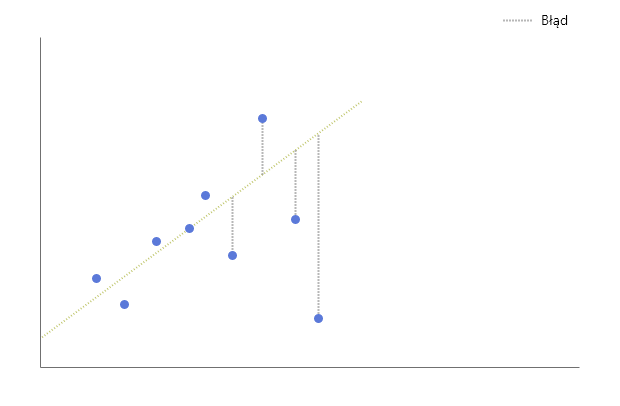
\includegraphics[scale=0.7]{linear_reg}
  \end{center}
  \caption{Wyznaczenie prostej regresji dla zbioru danych}
\end{figure}

\chapter{Projekt inzynierski}

\section{Opis architektury}
\subsection{Specyfikacja danych wejściowych}
Zbiór danych, który zostanie wykorzystany do zrealizowania zadania odnajdywania obserwacji odstających jest przedstawiony w uporządkowanej strukturze, która na potrzeby pracy została przeorganizowana (niektóre pola zostały usunięte ze względu na ich nieużyteczność) oraz przeredagowana (wartości niektórych pól zostały podmienione - na podstawie wcześniej stworzonego słownika - w celu ukrycia informacji wrażliwych). Dodatkowo powstało kilka struktur pomocniczych.
\\

\subsubsection{raw\_data}
Zbiór wszystkich punktów wartości, które zostały zmierzone. Jest to podstawowa struktura, z której danej posłużą wyszukiwaniu obserwacji odstających. Struktura ta zawiera wszystkie, nieprzypisane dane. Proces przypisywania i wyodrębniania danych, które dotyczą tego samego źródła zachodzi na bieżąco w czasie działania algorytmu. Tworzenie osobnych struktur (tabel w bazie danych) dla każdego źródła osobno byłoby mało optymalne i nieelastyczne (np. w sytuacji gdy dochodzą nowe "paczki" danych).
\\

\begingroup
\fontsize{10pt}{12pt}\selectfont

\begin{tabu} to 0.9\textwidth { | X[l] | X[l] | X[l] | X[l] | X[l] |}
\hline
\textbf{operator\_id} & \textbf{acronym} & \textbf{kpi\_name} & \textbf{date} & \textbf{value}\\
\hline
\textit{Long}  & \textit{Text}  & \textit{Text} & \textit{Timestamp} & \textit{Long} \\
\hline
364 & CANADA\_818 & KPI\_1 & 2015-10-30 10:45 UTC & 93.31 \\
\hline
\end{tabu}
\endgroup
\\
\\

\noindent \textbf{operator\_id} - numer identyfikujący operatora, którego dane dotyczą
\\\\
\textbf{acronym} - logiczny identyfikator wskazujący na pochodzenie danych (określający fizyczną lokalizację źródła danych)
\\\\
\textbf{kpi\_name} - nazwa określająca rodzaj urządzenia, które pomiar wykonało. Urządzenie to posiada dodatkowe cechy takie jak jednostka, co jest mierzone (jaki typ danych), jednak nie zostało to w tej strukturze uwzględnione, gdyż proces przetwarzania danych wymaga bardziej skomplikowanych definicji. Zostało to uwzględnione w dalszych strukturach danych.
\\\\
\textbf{date} - punkt w czasie, w którym pomiar został przeprowadzony. Może być to dokładna data lub data wskazująca na zakres dat (np. jeden dzień)
\\\\
\textbf{value} - wartość liczbowa dla tego punktu w danym czasie (tak samo jak dla daty, może to być wartość dla konkretnego punktu w czasie lub uśredniona wartość zebranych wartości z konkretnego okresu czasu).
\\ \\
Przykładową strukturę oraz źródła pochodzenia reprezentuje poniższy rysunek.
\begin{figure}[H]
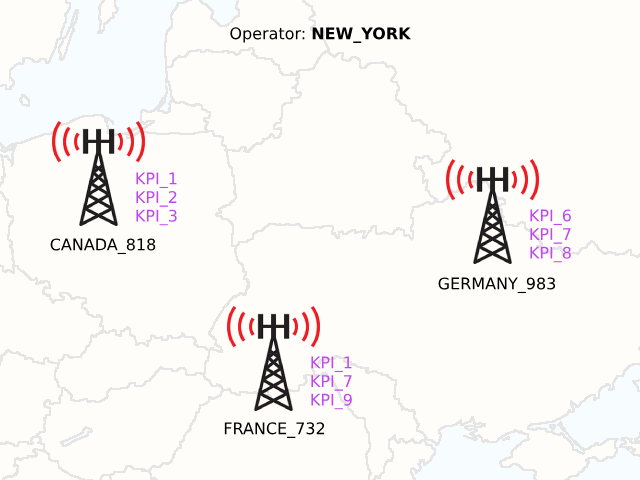
\includegraphics[scale=0.6]{struct}
\caption{Przykładowa struktura podziału sieci}
\end{figure}

Powyższa struktura w bazie danych wyglądałaby następująco:
\\\\
\begingroup
\fontsize{10pt}{12pt}\selectfont
\begin{tabu} to 0.9\textwidth { | X[l] | X[l] | X[l] | X[l] | X[l] |}
\hline
\textbf{operator\_id} & \textbf{acronym} & \textbf{kpi\_name} & \textbf{date} & \textbf{value}\\
\hline
364 & CANADA\_818 & KPI\_1 & 2015-10-30 00:00 UTC & 120.72 \\
\hline
364 & CANADA\_818 & KPI\_2 & 2015-10-31 00:00 UTC & 90.81 \\
\hline
364 & CANADA\_818 & KPI\_3 & 2015-11-01 00:00 UTC & 1483 \\
\hline
364 & FRANCE\_732 & KPI\_1 & 2015-10-30 00:00 UTC & 112.21 \\
\hline
364 & FRANCE\_732 & KPI\_7 & 2015-10-31 00:00 UTC & 121.2 \\
\hline
364 & FRANCE\_732 & KPI\_9 & 2015-11-07 00:00 UTC & 910.01\\
\hline
364 & GERMANY\_983 & KPI\_6 & 2015-10-31 00:00 UTC & 0 \\
\hline
364 & GERMANY\_983 & KPI\_7 & 2015-11-10 00:00 UTC & -1 \\
\hline
364 & GERMANY\_983 & KPI\_8 & 2015-12-29 00:00 UTC & 0.11 \\
\hline
\end{tabu}
\endgroup
\\

\subsubsection{kpi\_definitions}
Zbiór pomocniczy opisujący podstawowe cechy KPI. Zbiór ten nie wpływa na wyniki badań, może być jednak pomocny w procesie decyzyjnym (decyzja o uznaniu punktów odstających jako błędnych oraz usunięciu lub poprawieniu ich). W sytuacji gdy zbiór punktów określany przez definicję jest wyrażony w procentach decyzję o usunięciu / poprawieniu punktów można oprzeć na prostym założeniu, że punkty poza zakresem 0 - 100 są uznawane jako błędne.
\\

\begingroup
\fontsize{10pt}{12pt}\selectfont

\begin{tabu} to 0.9\textwidth { | X[l] | X[l] | X[l] | }
 \hline
 \textbf{formula} & \textbf{title} & \textbf{description}\\
 \hline
 \textit{Text}  & \textit{Text}  & \textit{Text} \\
\hline
 [KPI\_1/ 1000]  & Call interrupt measure  & Number of interrupted calls during the day \\
\hline

\end{tabu}
\endgroup
\\\\

\noindent\textbf{formula} - matematyczna formuła (równanie) złożona z jednego lub wielu \textit{kpi\_name}. Określa jak należy liczyć i interpretować wartości końcowe (np. jeden operator obserwuje zachowanie się sieci w różnych punktach geograficznych a następnie interpretuje średnią wartość jako wartość poprawną dla obszaru, który znajduje się w zasięgu sieci). Na potrzeby pracy formula składa się \textbf{z tylko jednego} kpi\_name, toteż dodatkowe przeliczenia nie są potrzebne co stanowczo uproszcza proces agregacji i wyszukiwania.
\\\\
\textbf{title} - tytuł definicji, używany jedynie dla lepszej reprezentacji danych po stronie użytkownika.
\\\\
\textbf{description} - krótki opis definicji, określający jakiego typu danych dotyczy przeprowadzony pomiar.

\subsubsection{operators}
Zbiór danych w postaci prostego słownika określającego nazwę operatora oraz jego unikalny identyfikator. Użyty w procesie początkowej anonymizacji danych.
\\

\begingroup
\fontsize{10pt}{12pt}\selectfont

\begin{tabu} to 0.9\textwidth { | X[l] | X[l] | }
 \hline
 \textbf{operator\_id} & \textbf{operator\_name}\\
 \hline
 \textit{Long}  & \textit{Text} \\
\hline
 364  & NEW\_YORK \\
\hline
\end{tabu}
\endgroup
\\\\

\noindent\textbf{operator\_id} - unikalny identyfikator operatora
\\\\
\textbf{operator\_name} - przyjazna użytkownikowi nazwa operatora. Podmieniona na nazwę losowego miasta w procesie anonymizacji.


\subsubsection{operator\_to\_acronym\_kpi}
Zbiór danych określający wszystkie występujące kombinacje trójki \textit{operator, acronym, kpi\_name}. Stworzenie tej struktury wynikało ze specyfiki użytej bazy danych (Cassandra DB), która wymaga podania wszystkich trzech kluczy do otrzymania pozostałych wartości wiersza.
\\
\begingroup
\fontsize{10pt}{12pt}\selectfont

\begin{tabu} to 0.9\textwidth { | X[l] | X[l] | X[l] | }
 \hline
 \textbf{operator\_id} & \textbf{acronym} &\textbf{kpi\_name}\\
 \hline
 \textit{Long}  & \textit{Text}  & \textit{Text} \\
\hline
 364  & CANADA\_818 & KPI\_1\\
\hline
\end{tabu}
\endgroup
\\\\

\subsubsection{acronym\_aliases}
Analogiczna struktura do \textit{operator\_aliases} jednak tycząca się rzeczywistych wartości dla \textit{acronym}. Za aliasy posłużyły nazwy krajów.
\\
\begingroup
\fontsize{10pt}{12pt}\selectfont

\begin{tabu} to 0.9\textwidth { | X[l] | X[l] | }
 \hline
 \textbf{raw} & \textbf{alias}\\
 \hline
 \textit{Text}  & \textit{Text} \\
\hline
 LTE\_818  & CANADA\_818 \\
\hline
\end{tabu}
\endgroup
\\\\

\subsection{Pochodzenie danych wejściowych}
Powyższe zbiory / struktury danych są rezultatem zbierania i agregowania danych z wielu źródeł jednocześnie. Dodatkowo dane otrzymane od firmy zostały wcześniej maszynowo uporządkowane (poprzez wykorzystanie licznych narzędzi i algorytmów). Wykorzystane dane w pracy nie są zatem otrzymane bezpośrednio. Tak duża różnorodność oraz ilość podejmowanych w stosunku do tych danych działań skutkuje licznymi błędami w nich (błędy, których wykrycie jest zadaniem niniejszej pracy). Z pośród wielu przyczyn tych błędów można wskazać kilka najczęściej występujących:
\begin{itemize}
\item \textbf{Błąd ludzki} - duży procent "paczek" danych jest przetwarzanych, sortowanych, dopasowywanych do odpowiednich baz danych przez ludzi. Dodatkowo często dochodzi do nieporozumień na etapie uzgadniana wartości i procesów biznesowych. Rezultatem tego są - zazwyczaj - długie przedziały niepasujących danych (trudniejsze do wykrycia maszynowo bez dodatkowych informacji ze względu na utrzymujący się trend).
\item \textbf{Błąd w algorytmach} - otrzymane dane zostały wzięte z jednej z wielu baz wykorzystywanych w firmie. Dane te często są częściowo lub w całości skopiowane z bazy innego systemu, który wykorzystuje wiele algorytmów dopasowywania danych w odpowiednie miejsca. Istnieją przypadki gdzie bazując na słownikach występuje decyzja o przypisaniu danych np. do odpowiedniego operatora, bardzo często zawierając instrukcje warunkowe, które nieaktualizowane z czasem powodują złe przypisania (zazwyczaj pojedyncze punkty).
\item \textbf{Uszkodzenia mechaniczne urządzeń} - możliwym przypadkiem są również wszelkiego rodzaju uszkodzenia sieci. Raportowane wówczas dane zawierają wszelkiego rodzaju przekłamania, różnice okresowe (zazwyczaj krótkie okresy).
\end{itemize}
\subsection{Specyfikacja danych wyjściowych}
Przetworzone przez algorytmy zbiory danych zostaną poetykietowane i posegregowane na dwa zbiory punktów:
\begin{itemize}
\item Punkt odstający - potencjalny punkt odstający swoją wartością od pozostałych z tego samego zbioru
\item Punkt poprawny - punkt sklasyfikowany jako należący do zbioru (punkt nieodstający)
\end{itemize}

Reprezentacja w bazie danych wygląda następująco:
\\
\begingroup
\fontsize{10pt}{12pt}\selectfont

\begin{tabu} to 0.9\textwidth { | X[l] | X[l] | X[l] | X[l] | X[l] | X[l] |}
\hline
\textbf{operator\_id} & \textbf{acronym} & \textbf{kpi\_name} & \textbf{date} & \textbf{value} & \textbf{is\_outlier}\\
\hline
\textit{Long}  & \textit{Text}  & \textit{Text} & \textit{Timestamp} & \textit{Long} & \textit{Boolean}\\
\hline
364 & CANADA\_818 & KPI\_1 & 2015-10-30 10:45 UTC & 93.31 & True\\
\hline
\end{tabu}
\endgroup

\subsection{Przeznaczenie danych wyjściowych}
Z powodu braku konkretnych informacji dodatkowych opisujących zachowanie się sieci czy specyfiki zbiorów danych wykryte obserwacje odstające można jedynie przekazać do dalszej analizy.\\
Rezultaty oczywiście mogą zostać przeprocesowane metodami do usuwania i korekcji danych jednak w tym przypadku nie ma żadnej pewności, że rezultat będzie poprawny czy w ogóle pożądany, bowiem charakterystyka danych jest na tyle specyficzna, że bez równie specyficznej wiedzy nie ma stu procentowej pewności na zgodność z oczekiwaniami.

\section{Aplikacja internetowa}
W celu analizy i przeprowadzania pojedynczych testów w łatwy i szybki sposób została stworzona aplikacja internetowa z poziomu której można wybrać konkretne zbiory danych oraz uruchomić algorytmy z zadeklarowanymi metodami wyszukiwania obserwacji odstających. Aplikacja dodatkowo umożliwia analizę oraz wizualizację zbiorów danych wraz z narzuconymi na wykres punktami sklasyfikowanymi jako odstające.
\subsection{Struktura aplikacji}
Aplikacja została podzielona na trzy główne warstwy, które komunikują się ze sobą oraz wymieniają dane za pomocą zapytań HTTP. Schemat komunikacji w prostu sposób ilustruje poniższy rysunek:

\begin{figure}[H]
  \begin{center}
  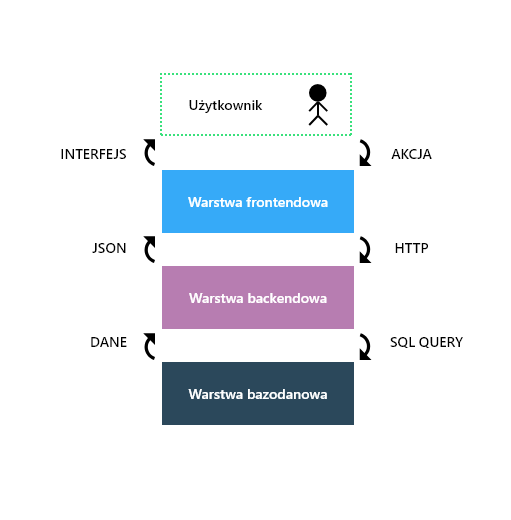
\includegraphics[scale=0.7]{layers}
  \end{center}
  \caption{Schemat komunikacji między warstwami aplikacji}
\end{figure}

\subsubsection{Warstwa frontendowa}
Warstwa odpowiedzialna za dostarczenie użytkownikowi informacji (danych) w graficzny sposób w przeglądarce internetowej. Dostarcza interfejs graficzny, który implementuje interaktywne elementy za pomocą, których generowane są zapytania do warstwy backendowej. Ze względu na jedynie pomocniczą rolę aplikacji internetowej w całym projekcie warstwa ta jest ograniczona do niezbędnego minimum.
\\\\
W projekcie warstwa frontendowa odpowiada za dostarczenie możliwości wyboru  kluczy identyfikujących zbiór danych a następnie po otrzymaniu danych w odpowiedzi zwrotnej wysłanego zapytania do warstwy backendowej wyświetla zbiór punktów w formie kartezjańskiego układu współrzędnych.
\subsubsection{Warstwa backendowa}
Warstwa niewidoczna dla użytkownika, obsługuje zdarzenia po stronie serwera nasłuchując i odbierając zapytania HTTP. Jest też bezpośrednio połączona z systemem bazodanowym. Zarządza danymi zapisanymi w notacji JSON (Javascript Object Notation) \cite{JSON}. Zadaniem tej warstwy jest uruchamianie procesów, o które warstwa frontendowa wysyła zapytania takie jak dostarczanie zbiorów danych oraz uruchamianie algorytmów wyszukiwania obserwacji odstających.
\\\\
Dodatkowym zadaniem warstwy bazodanowej jest uzupełnianie tabel w bazie danych na podstawie wcześniej zdefiniowanych słowników. Dzięki temu mając jedynie surowe dane dostarczone z zewnątrz cała struktura potrzebna do działania aplikacji może zostać odtworzona automatycznie.
\subsubsection{Warstwa systemu bazy danych}
Struktura fizyczna również umieszczona na serwerze dostarczająca informacje o zaimplementowanych strukturach danych oraz wartości przechowywanych w niej. Baza danych stanowi integralną cześć projektu.
\subsection{Języki programistyczne}
Podstawowym językiem wykorzystanym w warstwie frontendowej jest język Javascript \cite{js} w standardzie EcmaScript 6 \cite{es6} oraz składni TypeScript\cite{ts}, która zapewnia większą kontrolę nad strukturą kodu dostarczając niedostępne w podstawowej wersji Javascript typów zmiennych. W celu dostarczenia użytkownikowi przejrzystego interfejsu graficznego wykorzystany został język znaczników HTML 5(Hyper Text Markup Language)\cite{html} oraz CSS 3 (Cascading Style Sheets) \cite{css}.
\\\\
Warstwa backendowa jest napisana w języku python \cite{python}. Wybór tej technologi podyktowany jest głównie chęcią zbudowania jednolitego środowiska dla aplikacji oraz zaimplementowanych algorytmów uczenia maszynowego. Dzięki temu komunikacja i rozbudowa programu / aplikacji jest dużo prostsza.
\\\\
Jako system bazodanowy została wybrana Cassandra DB \cite{cassandra} ze względu na jest przystosowanie do obsługi  dużej ilości danych oraz prostej implementacji w języku python. Cassandra zapewnia szybki dostęp do dużej ilości danych jednocześnie.
\subsection{Wykorzystane rozwiązania}
\subsubsection{React.js}
\small \textbf{Wersja:} 16.8.3\\
React.js \cite{react} jest to jedno z najpopularniejszych rozwiązań przy tworzenie warstw frontendowych aplikacji. Wykorzystuje koncepcję komponentów i modularności. Jest napisany w języku JavaScript.
\subsubsection{React vis}
\small \textbf{Wersja:} 1.11.6\\
Biblioteka generująca zestawy wykresów na podstawie podanego zbioru danych. Dzięki niej możliwe jest zwizualizowanie konkretnych zbiorów danych oraz ingerencja w ich zachowanie (zmiana skali, zmiana kolorów punktów bazując na dostarczonych parametrach).
\subsubsection{Axios}
\small \textbf{Wersja:} 0.18.0\\
Biblioteka dostarcza podstawowe narzędzia do generowania zapytań HTTP. Ma zintegrowaną i rozwiniętą mechanikę obsługi błędów co czyni ją lepszą alternatywą niż wykorzystanie wbudowanej  w język Javascript metodyki \textit{fetch}.
\subsubsection{Lodash}
\small \textbf{Wersja:} 4.17.11\\
Biblioteka dostarcza szereg funkcji używanych do zarządzania obiektami w języku Javascript, ich organizacji oraz transformacji.
\subsubsection{Preprocessor SASS}
\small \textbf{Wersja:} 0.23.1\\
Preprocessor SASS jest językiem nadrzędnym nad CSS i jest do niego kompilowany. Dostarcza dodatkowe możliwości zarządzania atrybutami i zmiennymi w środowisku CSS co upraszcza i usprawnia proces tworzenia aplikacji.
\subsubsection{Falcon}
\small \textbf{Wersja:} 0.18.0\\
Paczka służąca do stworzenia serwera HTTP w środowisku python. Obsługuje podstawowe zadania tworzenia tzw. endpointów, czyli wcześniej zdefiniowanych ścieżek w postaci adresu HTTP, w których zaimplementowane jest obsługa takich zdarzeń jak GET, POST, PUT. Mechanizm ten jest wykorzystywany do komunikacji z warstwą frontendową.
\subsubsection{Click}
\small \textbf{Wersja:} 0.18.0\\
Paczka pozwalająca na proste tworzenie CLI (Command Line Interface), czyli konsolowego interfejsu, z poziomu którego za pomocą zdefiniowanych komend uruchamia się pojedyncze zadania.
\subsubsection{Figgypy}
\small \textbf{Wersja:} 0.18.0\\
Paczka wykorzystywana do zarządzania globalną konfiguracją serwera. Dostarcza zestaw parserów, która wcześniej zdefiniowane wartości zapisane w pliku tekstowym jest w stanie zinterpretować i dostarczyć odpowiednie wartości do wykonywalnego kodu. Plik konfiguracyjny zawiera m.in parametry połączenia z bazą danych (nazwa użytkownika, hasło itp).
\subsubsection{Cassandra driver}
\small \textbf{Wersja:} 0.18.0\\
Paczka obługujące połączenie bazodanowe z systemem bazy danych Cassandra DB. Odpowiada za nawiązywanie i zrywanie połączeń oraz tworzenie tzw. query, na podstawie których otrzymywane są żądane dane z bazy danych.
\subsection{Wykorzystane narzędzia}
Do poprawnego uruchomienia, tworzenia i działania aplikacji potrzebny jest szereg narzędzi programistycznych.
\subsubsection{NPM (Node Package Manager), Yarn}
Node Package Manager (NPM) oraz Yarn są to podobne narzędzia. Służą one do zarządzania zależnościami (paczkami, bibliotekami) warstwy frontendowej. Za ich pomocą można instalować nowe paczki, aktualizować już istniejące czy usunąć je z projektu.
\subsubsection{Pipenv}
Odpowiednik NPM / Yarn dla warstwy backendowej. Pipenv jest nadrzędnym narzędziem biblioteki pip oraz virtenv. Poza zarządzniem zależnościami i paczkami pipenv również tworzy wirtualne środowisko programistyczne dla języka python.
\subsubsection{TS Lint, SASS Lint, Prettier}
Zestaw narzędzi, który pozwala na utrzymanie kodu aplikacji w uporządkowany sposób za pomocą ustalonych wcześniej reguł. Dodatkowo implementują one narzędzia automatyzujące proces formatowanie kodu.
\subsubsection{Webpack}
Narzędzie zarządzające transformacją kodu warstwy frontendowej. Transformuje język wyższego rzędu (es6 oraz Typescript) na język Javascript zrozumiały dla współczesnych przeglądarek. Dodatkowo optymalizuje rozmiar plików skryptowych a także dostarcza narzędzia programistyczne takie jak testowy serwer czy walidacja kod uw czasie rzeczywistym.
\subsubsection{GIT, Github}
GIT jest to system kontroli wersji dostępny z poziomu konsoli. Tworzy lokalne repozytorium zawierające kod aplikacji. Zapewnia bezpieczeństwo kodu i szybki dostęp do zapisanych zmian.
\\\\
Github jest to aplikacja webowa, która dostarcza zdalne repozytorium (zintegrowany z lokalnym) co zapewnia dostęp do napisanego kodu niezależnie od miejsca. Zapewnia też podstawowy system kopii zapasowej.
\subsubsection{Docker}
Narzędzie pozwalające na prostą konfigurację oraz uruchamianie aplikacji (tu: bazy danych) na każdym środowisku.
\subsection{Wymagania funkcjonalne}
\subsubsection{Wybór kluczy zbioru danych}
\textbf{Nr wymagania:} 1 
\\\\
\textbf{Przesłanka}\\
Aby otrzymać dane żądanego zbioru danych i je wyświetlić należy wybrać zestaw składający się z trzech kluczy reprezentujących zbiór danych.
\\\\
\textbf{Opis}\\
\textbf{Warstwa frontendowa} \\
Użytkownik ma do wyboru trzy selektory:
\begin{itemize}
\item Operator
\item Akronim
\item KPI Name
\end{itemize}

Wszystkie selektory poza selektorem operatora są zablokowane. Selektory odblokowują się po wyborze wartości w selektorze poprzednim zgodnie z powyższą hierarchią. Zapewniany jest tym sposobem dostęp do danych, które są reprezentowane przez wybrane klucze. Po wyborze wartości w ostatnim selektorze (KPI Name) wysyłane jest żądanie do warstwy backendowej. 
\\\\
\textbf{Warstwa backendowa}
Po odebraniu żądania z zawartymi informacjami o kluczach w formacie JSON wysyłane jest zapytanie do bazy danych a następnie zwracane wszystkie otrzymane wartości. Dane te są wyświetlane przez warstwę frontendową zgodnie z wymaganiem nr. 2.
\\\\\noindent\rule{\textwidth}{2pt}
\subsubsection{Wyświetlanie danych w formacie wykresu w układzie kartezjańskim}
\textbf{Nr wymagania:} 2
\\\\
\textbf{Przesłanka}\\
Wyświetlanie danych w graficzny sposób pozwala na lepszą analizę zbioru danych.
\\\\
\textbf{Opis}\\
\textbf{Warstwa frontendowa} \\
Po otrzymaniu punktów wybranego zbioru danych na ekranie aplikacji pojawia się wykres składający się z dwóch osi:
\begin{itemize}
  \item Oś X - Czas w postaci stempla czasowego
  \item Oś Y - Numeryczna wartość punktu 
\end{itemize}
Punkty zaznaczone są w postaci jednolitych kropek połączonych prostymi liniami. Wykres można dopasować do okna przeglądarki lub rozciągnąć wraz z zastosowaniem suwaka poziomego. Połączenia między punktami można ukryć lub pokazać na żądanie użytkownika.
\\\\\noindent\rule{\textwidth}{2pt}
\subsubsection{Uruchamianie metod wyszukiwania obserwacji odstających}
\textbf{Nr wymagania:} 3
\\\\
\textbf{Przesłanka}\\
Wybrane i uruchomienie metody wyszukiwania obserwacji odstających stanowi podstawę projektu i jest niezbędne do analizy i realizacji celu pracy.
\\\\
\textbf{Opis}\\
\textbf{Warstwa frontendowa}\\
Po wyborze i wyświetleniu zbioru danych dostępna jest możliwość wyboru zdefiniowanej i zaimplementowanej metody wyszukiwania obserwacji odstających. PO zatwierdzeniu tej operacji wysyłane jest żądane do warstwy backendowej.
\\\\
\textbf{Warstwa backendowa}\\
Po otrzymaniu zapytania o uruchomienie żądanej metody wraz z kluczami zbioru danych wysyłane jest zapytanie o dane do bazy danych a następnie uruchamiania jest wymagana metoda. Niezależnie od metody po skończeniu działania algorytmu danymi wyjściowymi jest cały zbiór danych z dodatkowo dołączoną informacją do każdego punkty o tym, czy jest on potencjalnym punktem odstającym (w formie Boolean: True / False). Tak zmodyfikowany zbiór danych jest zwracany do warstwy frontendowej.
\\\\\noindent\rule{\textwidth}{2pt}
\subsubsection{Nanoszenie punktów odstających na wykres}
\textbf{Nr wymagania:} 4
\\\\
\textbf{Przesłanka}\\
Wizualizacja miejsc, w których punkty odstające zostały znalezione pozwala lepiej przeanalizować i zrozumieć działanie wybranych metod i algorytmów.
\\\\
\textbf{Opis}\\
\textbf{Warstwa frontendowa}\\
Po zwróceniu zmodyfikowanych danych przez warstwę backendową zgodnie z wymaganiem nr. 4 tworzony jest wykres tą samą metodą co w wymaganiu nr. 2 z modyfikacjami koloru dotyczących punktów:
\begin{itemize}
  \item punkty z informacją w dodatkowym polu równą True na czerwono
  \item pozostałe punkty na szaro
\end{itemize}
\section{Implementacja metod i algorytmów}
\subsection{Wykorzystane technologie}
\subsubsection{numpy} 
Duża biblioteka zawierająca zaawansowane metody do zarządzania matematycznymi strukturami danych takich jak macierze, wektory. Bilbioteka pozwala na prosty sposób zarządzania transformacjami danych pod kątem użycia ich w algorytmach dostarczonych przez scikit-learn. \cite{numpy}
\subsubsection{scikit-learn} 
Bilbioteka dostarczająca algorytmy uczenia maszynowego wykorzystywane w pracy.  \cite{scikit-learn}
\subsection{Przygotowanie zbioru uczącego}
Posiadane dane oprócz kluczy zawierają zaledwie dwie cechy - czas i wartość. Obie z tych cech są cechami słabymi ze względu na ich zbyt duży rozrzut i dużą unikalność - stempel czasowy jest inny dla każdego punktu a rozrzut wartości często jest bardzo duży (dodatkowo wartości bardzo często są równie unikatowe co czas). \\
Aby proces uczenia maszynowgo przez wybrane algorytmy był trochę bardziej efektywny został zaimplementowany algorytm, który dopasuje i doda dodatkową cechę bazującą na stemplu czasowym. Zostały zaimplementowane trzy takie cechy - do wyboru w zależności od zbioru danych:
\begin{itemize}
	\item dzien miesiaca (np. 28 dzien miesiaca to cecha 28)
	\item dzien tygodnia (np. wtorek to cecha 2)
	\item kombinacja dnia miesiące i samego miesiąca (np. 09.05 to cecha 0905)
\end{itemize}
Powoduje to, że w zależności od wybranej cechy można zwiększyć podobieństwo punktów do siebie. 
\\\\
Wybranie tych cech idzie łącznie z założeniem, że zbiór danych posiada jakikolwiek trend. Przykładowy kod ustalający dodatkową cechę może być zaimplementowany w poniższy sposób:
\\
\begin{lstlisting}
 def get_dataset_with_day_feature(self, feature):
        dataset_with_day = self.dataset
        for index, data in enumerate(dataset_with_day):
            daytime_timestamp = datetime.fromtimestamp(data['timestamp'])
            if feature == 'day':
                day = daytime_timestamp.day

            if feature == 'monthday':
                day = "{}{}".format(daytime_timestamp.day, daytime_timestamp.month)

            if feature == 'weekday':
                day = daytime_timestamp.weekday()

            if feature == 'timestamp':
                day = data['timestamp']

            dataset_with_day[index]['day'] = int(day)

        return dataset_with_day
\end{lstlisting}

Końcowa strutkura pojedynczego punktu wygląda zatem następująco:
\\
\begingroup
\fontsize{10pt}{12pt}\selectfont

\begin{tabu} to 0.9\textwidth { | X[l] | X[l] | X[l] |}
\hline
\textbf{value} & \textbf{timestamp} & \textbf{feature} \\
\hline
\textit{Long}  & \textit{Long}  & \textit{Long} \\
\hline
\end{tabu}
\endgroup

\subsection{Algorytm uruchamiania metody w pętli}
Ze względu na pewną losowość wykorzystanych algorytmów uczenia maszynowego jednokrotne uruchomienie algorytmów na zbiorze danych może nie być jednoznacznie rozstrzygające (nigdy nie będzie, jednak można zwiększyć jego wiarygodność) został zaimplementowany algorytm uruchamiający jedną metodę wyszukiwania obserwacji odstających kilkukrotnie (w pętli). Ilość iteracji jest zadana z góry, niezmienność wyników została zaobserwowana w granicach 10 -15 razy. 
\\\\
Działanie pojedynczej iteracji można przedstawić w poniższy sposób:

\begin{itemize}
  \item uruchom przekazaną metodę wyszukiwania anomalii
  \item zapamiętaj zwrócone przez tę metodę punkty odstające
  \item w kolejnych iteracjach dodawaj wystąpienia lub nowe punkty (jeśli się pojawiły)
  \item sklasyfikuj jedynie punkty jako odstające jeśli wystąpiły w 80 procentach przypadków (dla 10 iteracji wszystkie punkty, który wystąpiły więcej niż 8 razy są uznawane za odstające)
  \item zwróć wynik
\end{itemize}

Algorytm można zaimplementować w następujący sposób:

\begin{lstlisting}
    def run_calculations(method):
        iterations = 10
        labeled_result = []
        outliers_prob = {}

        for iteration in range(0, iterations):
            labeled_result = method()

            point_with_outliers = list(filter(lambda p: p['is_outlier'], labeled_result))
            for point in point_with_outliers:
                try:
                    outliers_prob[point['id']] = outliers_prob[point['id']] + 1
                except KeyError:
                    outliers_prob[point['id']] = 1

        final_result = []
        for data_point in labeled_result:
            try:
                is_outlier = outliers_prob[data_point['id']] / iterations > 0.8
            except KeyError:
                is_outlier = False

            final_result.append({
                'id': data_point['id'],
                'value': data_point['value'],
                'timestamp': data_point['timestamp'],
                'day': data_point['day'],
                'is_outlier': is_outlier,
                'label': data_point['label']
            })

        return final_result
\end{lstlisting}


\subsection{Podział zbioru danych na okna czasowe}
Zgodnie z opisem w punkcie 2.1 algorytm podziału na okna czasowe można zaimplementować w poniższy sposób:
\begin{lstlisting}
import numpy as np


def create_windows(data, window_len, slide_len):
    chunks = []
    for pos in range(0, len(data), slide_len):
        chunk = np.copy(data[pos:pos + window_len])
        chunks.append(chunk)

    return chunks
\end{lstlisting}
\subsection{Metoda odległości od centroidów z wykorzystaniem algorytmu KMean}
Metoda opisana w punkcie 2.2.1 została w zaimplementowana w całości, z uwzględnieniem dwóch warunków definiowania punktu jako odstający. Wybór jednej z nich odbywa się na żądanie użytkownika. W procesie testowania metod oba warunki są używane w celu porównania ich działania.\\
Końcowe działanie metody można przedstawić na prostym przykładzie:
\\\\
Badaniu został poddany zbiór zawierający 30 punktów. Liczba klastrów została ustalona na 2. Podział wygląda następująco:
\begin{figure}[H]
  \begin{center}
    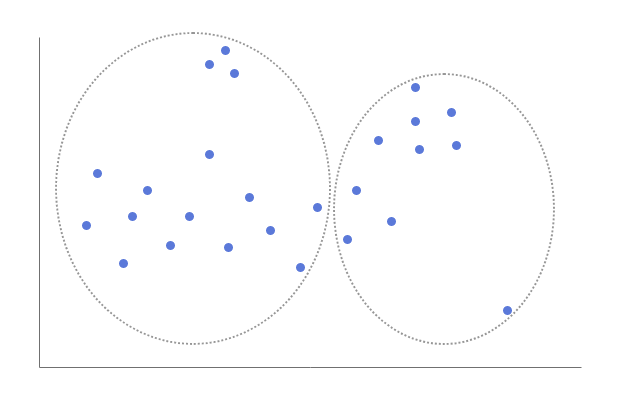
\includegraphics[scale=0.5]{kmean_dist}
        \caption{Podział zbioru danych na dwa klastry}
  \end{center}
\end{figure}
Zostały obliczone odległości od centroidów klastrów a następnie obliczone potrzebne miary:
\begin{itemize}
  \item[--] odległość każdego punktu od swojego centroidu
  \item[--] średnia odległość punktu od centroidu w klastrze
  \item[--] najmniejsza odległość punktu od centroidu w klastrze
\end{itemize}
\begin{figure}[H]
  \begin{center}
    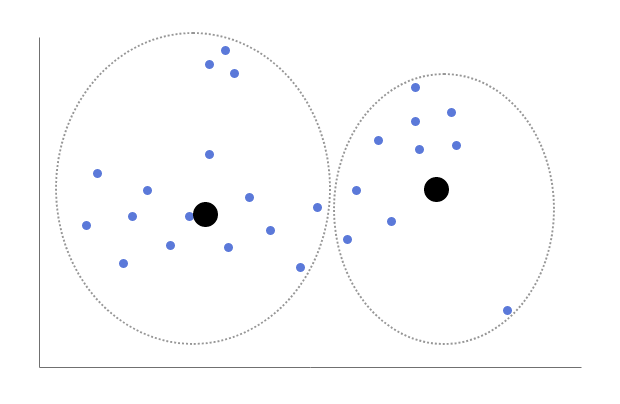
\includegraphics[scale=0.5]{kmean_dist_1}
        \caption{Podzielony zbiór danych z wyznaczonymi centroidami}
  \end{center}
\end{figure}
W zależności od wyboru metody punkty sklasyfikowane jako odstające po pierwszej iteracji zostały zaznaczone na czerwono.\\

\begin{figure}[H]
  \begin{center}
    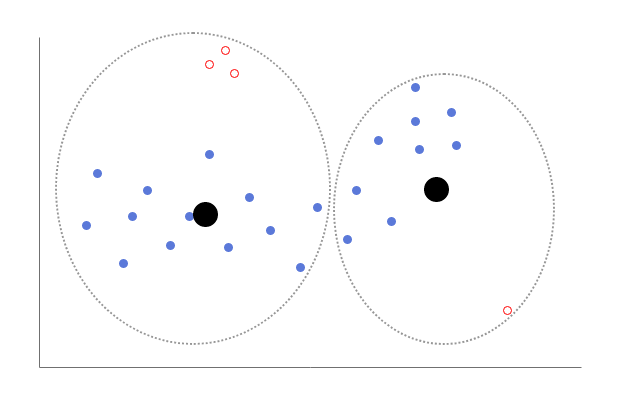
\includegraphics[scale=0.5]{kmean_dist_2}
    \caption{Punkty odstające wyznaczone przez odrzucenie punktów powyżej zadanego progu}
\end{center}

\begin{center}
  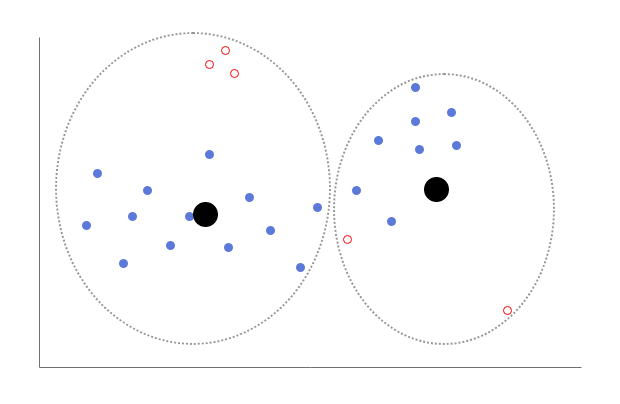
\includegraphics[scale=0.5]{kmean_dist_3}
  \caption{Punkty odstające wyznaczone przez odrzucenie 5 punktów najdalej oddalonych}
  \end{center}
\end{figure}
Powyższy przykład nie ilustruje rzeczywistego działania algorytmu. Przyjęto pewne uproszczenia i zaokrąglenia przy wyznaczaniu miar i punktów odstających.

\subsection{Metoda ilości punktów w klastrze z wykorzystaniem algorytmu KMean}
Metoda opisana w punkcie 2.2.2 została zaimplementowana zgodnie z opisem uwzględniając obliczenie parametrów, które są wymagane do obiczenia warunku (progu):
\begin{itemize}
	\item stosunek wielkości zbioru danych do ilości klastrów
	\item ilość punktów w każdym klastrze
	\item średniej liczby punktów na klaster
\end{itemize}
Znając powyższe parametry oraz zadany z góry warunek (próg) można zdefiniować równanie, na podstawie którego rozpatrywane są pojedyncze klastry:
\\
\begin{equation*}
LP = \lfloor W / 100\% \times SPK  \rfloor
\end{equation*}
gdzie,\\
$LP$ - Maksymalna liczba punktów w klastrze \\
$W[\%]$ - Zdefiniowany warunek \\
$SPK$ - Średnia liczba punktów na klaster \\
\\\\
Znając liczbę $LP$ oraz ilość punktów w każdym klastrze można sklasyfikować te klastry których liczba punktów jest $\le LP$
\\\\
Implementacja całej metody w kodzie może wyglądać następująco:

\begin{lstlisting}
import numpy as np
from sklearn.cluster import KMeans


def sim_kmean(n_clusters, dataset, similarity):
    filtered_dataset = np.array(list(map(lambda data: [data['value'], data['day']], dataset)))
    model = KMeans(n_clusters)
    clusterer = model.fit(filtered_dataset)
    labels = model.predict(filtered_dataset)
    centroids = clusterer.cluster_centers_

    labeled_result = dataset
    centroids_counter = {}

    for index, label in enumerate(labels):
        key = str(centroids[label][0])
        try:
            centroids_counter[key] = centroids_counter[key] + 1
        except KeyError:
            centroids_counter[key] = 1

    for index, label in enumerate(labels):
        key = str(centroids[label][0])
        labeled_result[index]['is_outlier'] = centroids_counter[key] <= similarity
        labeled_result[index]['label'] = int(label)

    return labeled_result
\end{lstlisting}

\subsection{Metoda regresji liniowej z wykorzystaniem podziału na okna czasowe}
Metoda polegająca na obliczanie obserwacji odstających za pomocą metody wyznaczenia linii regresji (opisana w punkcie 2.3) w każdym oknie czasowym wyznaczonym metodą opisaną w punkcie 2.1. Następnie przed przesunięciem okna i przystąpienia do kolejnej iteracji punkty sklasyfikowane jako odstające są zapamiętywane a ich wystąpienia zliczane (podobnie jak w metodzie opisanej w punkcie 3.3.2). Następnie po ostatniej iteracji zliczany jest stosunkowy procent wystąpienia punktu jako odstającego (ilość wystąpień / ilość iteracji(ilość okien)). Warunkiem klasyfikacji jest, podobnie jak w metodzie uruchamiania metody w pętli (3.3.3), próg 80 procent lub więcej. \\\\
Z racji tego, że samo działanie metody jest zbliżone do uruchamiania metod w pętli (3.3.3) łączenie tych dwóch podejść jest już zbędne.
\\\\
Działanie algorytmu można pokazać w następujący sposób:
\begin{figure}[H]
  \begin{center}
  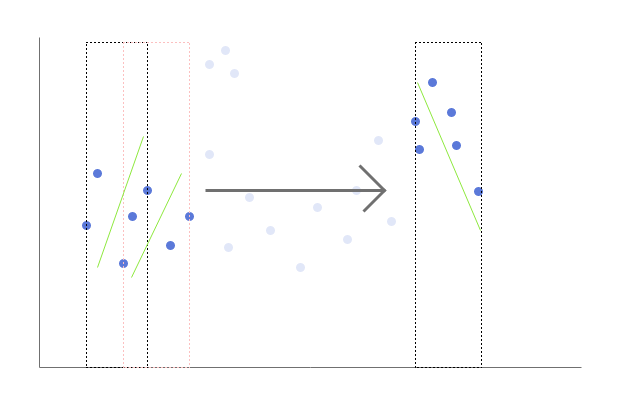
\includegraphics[scale=0.7]{reg_windowed}
  \end{center}
  \caption{Wyznaczenie prostych regresji dla zbioru danych podzielonego na okna}
\end{figure}
\chapter{Przeprowadzanie badań}
\section{Przygotowanie środowiska}
Pierwszym krokiem przeprowadzenia badań i testów jest przygotowanie śrdowiska wraz z implementacją. Należy wybrać metody wyszukiwania obserwacji odstających a następnie określić ich parametry jako zmienne lub stałe.
\\\\
Przed przystąpieniem do testów zostały wybrane tylko te zbiory danych, które zawierają więcej niż 800 pojedynczych punktów (dane z conajmniej dwóch lat). Dzięki temu wszystkie wybrane algorytmy powinny działać na takich samych zasadach (odpowiednia ilość punktów w klastrach a trend, jeśli istnieje, został już wyznaczony, możliwość dobrego podziału na okna czasowe).
\subsection{Wybór parametrów testowych}
Parametry testowe są to wszystkie parametry jakich wymaga metoda do poprawnego działania. Ze względu na dużą ilość danych parametry zmienne powinny przyjmować maksymalnie 3 różne wartości z różnego zakresu.\\
Z racji tego, że wielkości zbiorów danych są wybrane tak, aby ilość punktów zawierających się w nich była większa niż 700 można z góry narzucić pewne wartości parametrów bez zbędnego wyliczania ich indywidualnie dla każdego zbioru danych.
\\\\
Przyjęto kolejne parametry:\\
\textbf{Metoda odległości od centroidu (3.3.5)}
\begin{itemize}
	\item ilość klastrów: 20, 40
	\item wszystkie trzy dodatkowe cechy (3.3.2)
	\item oba warunki klasyfikacji (1.5 i 3 jako parametry warunku)
\end{itemize}
Ilość wykonanych uruchomień algorytmu na jednym zbiorze danych: 24
\\\\
\textbf{Metoda ilości punktów w klastrze (3.3.6)}
\begin{itemize}
	\item ilość klastrów: 20, 40
	\item wszystkie trzy dodatkowe cechy (3.3.2)
	\item dwa parametry dla warunku metody: 30 i 50 procent
\end{itemize}
Ilość wykonanych uruchomień algorytmu na jednym zbiorze danych: 12
\\\\
\textbf{Metoda regresji liniowej z oknem czasowym (3.3.7)}
\begin{itemize}
	\item wszystkie trzy dodatkowe cechy (3.3.2)
	\item dwa parametry dla warunku metody: 1.5 i 3
	\item dwie różne wersje parametrów okna czasowego: krok 2, szerokość okna 22 oraz krok 5, szerokość okna 50
\end{itemize}
Ilość wykonanych uruchomień algorytmu na jednym zbiorze danych: 12
\\\\
\subsection{Wybór zbiorów danych}
Docelowo wszystkie zbiory danych zostaną poddane badaniom, jednak wnioski zostaną oparte tylko na kilku wybranych. O wyborze zbioru będzie decydowała głównie jego charakterystyka oraz odmienność od innych. W końcowym podsumowaniu powinny się znaleźć zbiory bez oraz z mocno wyznaczonym trendem czy z wartościami mocno wahającymi się oraz z częstymi wygaśnięciami.\\
Specyfika oraz powód wyboru każdego wybranego zbioru zostanie opisana wraz z przedstawieniem jego wyników.
\section{Stworzenie programu automatyzującego}
Ważną częścią etapu uruchamiania testów i badań jest stworzenie programu, który w sposób automatyczny będzie w stanie uruchomić wcześniej zdefiniowane metody kolejno z różnymi parametrami. WYnika to z tego, że cały proces uruchamiania metod jest czasochłonny. Uruchamianie kolejno metod ręcznie jest możliwe, jednak nieoptymalne (brane jest pod uwagę ręczne uruchomienie pojedynczych testów tylko w momencie chęci potwierdzenia wyniku). 

\subsection{System zapisywania do bazy danych}
Program automatyzujący ma za zadanie uruchomić badanie / test a następnie zdefiniowane parametry końcowe zapisać w bazie danych. Końcowe parametry każdego pojedynczego testu to:
\begin{itemize}
	\item trzy klucze identyfikujące zbiór danych
	\item czas trwania (data rozpoczęcia i zakończenia)
	\item tablica identyfikatorów sklasyfikowanych punktów odstających
	\item parametry, z jakimi test został uruchomiony
\end{itemize}

\subsection{System raportowania}
Po przeprowadzeniu wszystkich zdefiniowanych testów zostanie uruchomiona procedura tworzenia raportów. Pojedynczy raport tyczy się jednego zbioru danych oraz metod jakie zostały na nim uruchomione. W skład tej procedury wchodzą:
\begin{itemize}
	\item agregacja sklasyfikowanych punktów odstających (ilość, wystąpienia, powtórzenia)
	\item agregacja czasów trwania pojedynczych testów (średni czas, najkrótszy, najdłuższy)
\end{itemize}
Pojedynczy raport jest zapisany jako tabela w formacie CSV.
\section{Wybór kryteriów porównania}
\section{Porównanie metod wyszukiwania obserwacji odstających}
\section{Wnioski}
\chapter{Podsumowanie i mowa końcowa}


\bibliography{bibliografia}
\end{document}